  $k$-kubkiem nazwiemy zbiór $k$ punktów na płaszczyźnie, takich że mają różną współrzędną $x$ i dla dowolnych dwóch z nich jest tak, że punkty ,,pomiędzy'' nimi (tzn. jeśli te dwa punkty mają jakieś współrzędne $x_1$, $x_2$ to wszystkie punkty o współrzędnych $x_j$ takich, że $x_1 < x_j < x_2$) są poniżej linii prostej puszczonej przez te dwa punkty. $k$-kubek składa się z $k$ punktów, które są w pozycji wypukłej (dowód przez ,,bo tak'').  Analogicznie $c$-czapeczką nazwiemy zbiór $c$ punktów na płaszczyźnie, bla bla bla, wszystkie punkty pomiędzy dwoma danymi punktami są ponad linią przechodzącą przez nie. Jak ktoś sobie to narysuje, to wyjdzie mu właśnie struktura czapeczkopodobna. To też jest w pozycji wypukłej. 

  Jako $f(k,c)$ będziemy oznaczać minimalną taką liczbę, że jeśli mamy $f(k,c)$ punktów o różnych współrzędnych $x$ na płaszczyźnie (i w pozycji ogólnej) to znajdziemy tam $k$-kubek lub $c$-czapeczkę. Wtedy też 
  \begin{theorem}[O kubkach i czapkach]
        Liczba $f(k,c)$ określona jest poprawnie.
    \end{theorem}
  \begin{proof}
    Indukcja po $k,c$. Widać trywialnie, że  $f(2,c) = 2$ oraz $f(k,2) = 2$. Pokażemy teraz ograniczenie górne na $f(k,c)$: \begin{equation*}
        f(k,c) \leq f(k-1,c) + f(k, c-1) - 1
    \end{equation*} 

    Rozważmy zbiór punktów w pozycji ogólnej o różnych współrzędnych $x$ mający $ f(k-1,c) + f(k, c-1) - 1 $ elementów. Nazwiemy go $P$. Z założenia indukcyjnego (biorąc pod uwagę pierwszy składnik) znajduje się w nim $k-1$-kubek lub $c$-czapeczka. Jeśli znajduje się tam $c$-czapeczka to od razu mamy sprawę załatwioną; zakładamy więc że jest tam $k-1$-kubek. Robimy teraz sobie zbiór $E$, taki że zawiera wszystkie końce $k-1$-kubków z $P$. Na pewno jest taki jeden (bo na pewno mamy $k$-kubek). Okazuje się jednak, że moc $E$ jest całkiem spora. Pokazujemy to za pomocą bardzo ciekawego fikołka; wywalamy ten koniec $k-1$-kubka o którym wiemy, że on istnieje ze zbioru $P$ (tak na chwilę). Plot twist polega na tym, że nadal mamy dostatecznie dużo punktów by zmajstrować $k-1$ kubek (być może zupełnie gdzie indziej, ale na pewno gdzieś on jest), bo punktów teraz jest $f(k-1,c) - 1 + f(k, c-1) - 1 \geq f(k-1,c)$. Procedurę tę powtarzamy póki możemy i wychodzi nam, że zbiór $E$ ma moc co najmniej $f(k,c-1)$. Fajnie. Teraz jeśli zbiór $E$ zawiera $k$-kubek to mamy tezę udowodnioną, więc załóżmy że zawiera $c-1$-czapeczkę. Biorę sobie teraz tę $c-1$-czapeczkę; jej pierwszy punkt jest równocześnie końcem jakiegoś $k-1$-kubka.
    
    To jest bardzo śmieszny moment, bo już jesteśmy blisko końca dowodu. Weźmy sobie punkt który stanowił koniec $k-1$-kubka i początek $c-1$-czapeczki. Nazwijmy go $y$. Punkt ,,na lewo'' od niego, przedostatni w kubku, nazwijmy $x$. Punkt ,,na prawo'' od niego, drugi w czapeczce, nazwijmy $z$. Rozpatrzmy prostą która idzie między punktami $x$ i $z$. Można dokonać szokującego odkrycia, że $y$ leży albo nad nią, albo pod nią (jeśli leży na niej to punkty nie znajdowały się w pozycji ogólnej, co przeczyłoby założeniom twierdzenia). Teraz jeśli $y$ leży pod nią, to ja mogę sobie rozszerzyć mój $k-1$-kubek na $k$-kubek, dorzucając do niego $z$, a jeśli nad, to mogę sobie analogicznie rozszerzyć czapeczkę. To kończy już dowód. 

    \begin{figure}[H]
        \centering
        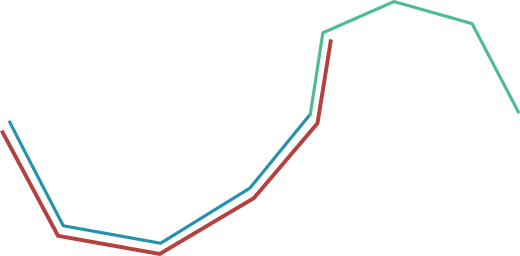
\includegraphics{images/k_kubek.png}
        \caption{Rozszerzanie kubka}
    \end{figure}

    
    \begin{figure}[H]
        \centering
        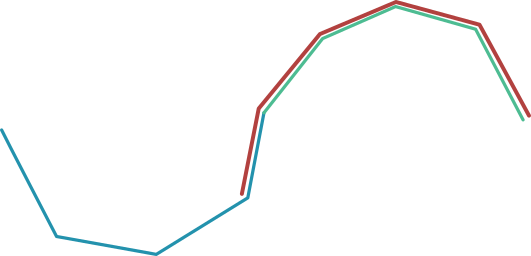
\includegraphics{images/k-czapka.png}
        \caption{Rozszerzanie czapki}
    \end{figure}
    
  \end{proof}